\documentclass[letterpaper,12pt]{texMemo}

\usepackage{graphicx}
\usepackage{setspace}
\usepackage{enumitem}
\usepackage{natbib}

\memoto{Bonnie Hsia, Professor}
\memofrom{Partha Sarathi Ghosh}
\memosubject{Comment on the 200W Course Learning Outcomes}
\memodate{\today}
%\logo{\includegraphics[width=0.3\textwidth]{Microsoft-Logo.pdf}}

\begin{document}
\begin{singlespacing}
\setlist[enumerate]{itemsep=0mm}
\maketitle

% Write me a memo in which you comment on the 200W Course Learning Outcomes that are listed on Page 3 of the syllabus:
%
% Write using a variety of technical writing and professional formats. (CLO#1)
% Compose with a clear focus on purpose, scope, and audience. (CLO#2)
% Document properly and provide accurately formatted references. (CLO#3)
% Locate and analyze information using a variety of research techniques (e.g., interviews, library, online searches). (CLO#4)
% Demonstrate an understanding of the initial planning, brainstorming, and organizing of a complex project. (CLO#5)
% In particular, I’m interested in your thoughts regarding these three questions:
%
% Which activities and assignments were particularly helpful in supporting these outcomes?
% What would you like to have done more of (or less of) in support of these outcomes?
% How have your capabilities changed in these five areas over the course of the semester?
% Please note:
%
% As I read your response to this assignment, I will—above all—be focusing on the quality of your writing rather than the content. In other words, I would like you to feel safe that you can tell me what you want to tell me in response to these questions versus telling me only positive things that you think I might want to hear.
% Please demonstrate to me that you know how to format a memo properly and that you can begin a memo telling its reader why he or she in particular is receiving the memo and what the purpose of the memo is.
% This memo should be one to two pages in length and single-spaced.
%In the opening paragraph of your memo or email, you should always tell your reader why he or she is receiving this email in particular and what the purpose is for the email. What this means is that your opening paragraph will probably be fairly short, possibly no more than one sentence or two.

% single or double spacing

%\doublespacing
% \begin{enumerate}
%     \item Identify all the physical and virtual assets in an organization.
%     \item Assign a risk profile to each asset.
%     \item Perform risk evaluation on each asset.
%     \item Perform risk mitigation on each asset.
% \end{enumerate}

% \begin{figure}[h!]
%     \centerline{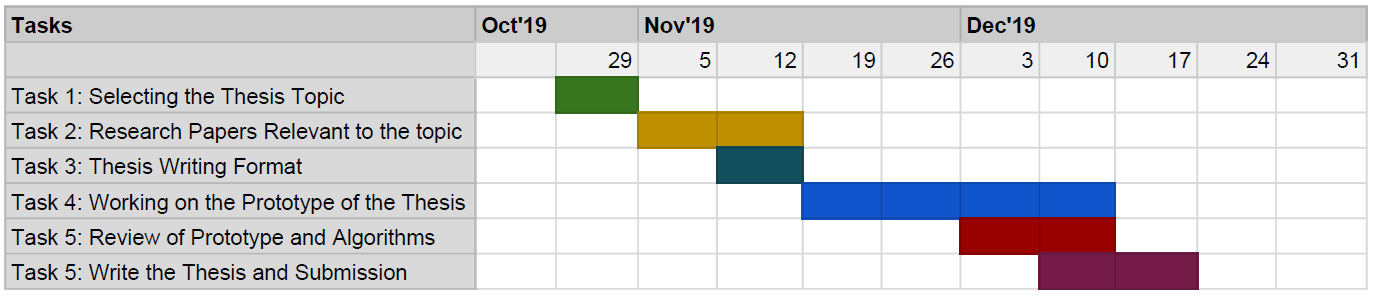
\includegraphics[scale=.45]{GaantChartThesis.PNG}}
%     \caption{Gantt Chart for Litearture Review}
%     %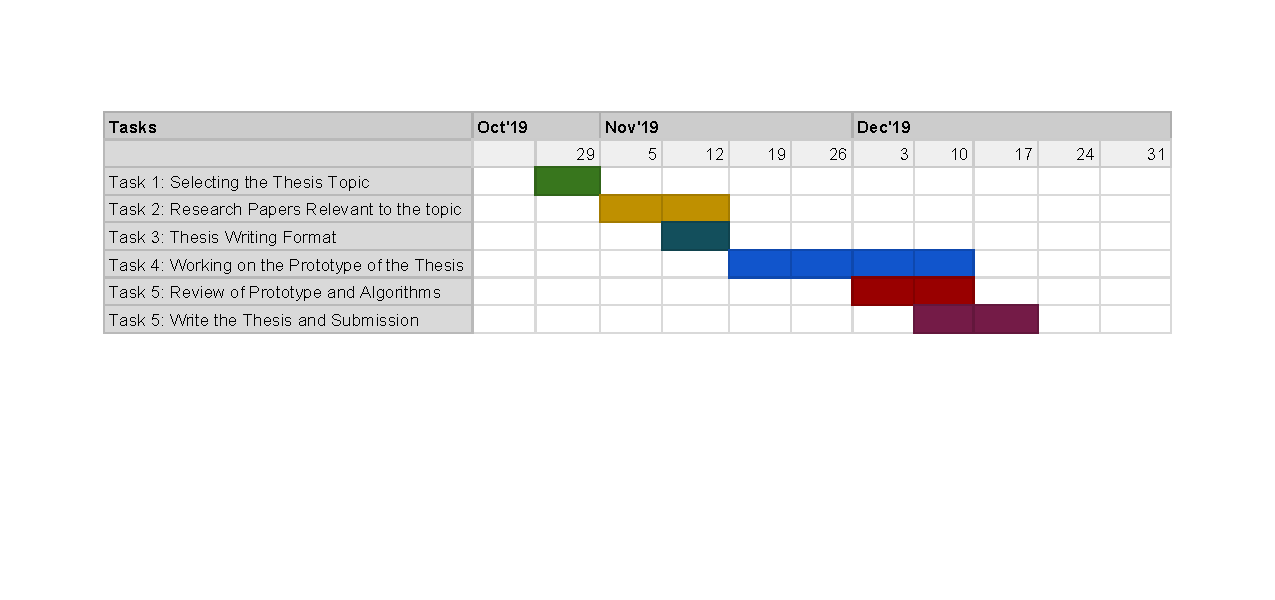
\includegraphics[scale=.8]{GaantChartThesis.pdf}
% \end{figure}

\section*{Purpose}
%This memo is for what ??
The purpose of this memo is to comment on the 200W Course Learning Outcomes (CLOs).


%%%%%%%%%%%%%%%%%%%%%%%%%%%%%%%
%PARTHA'S section starts here
%%%%%%%%%%%%%%%%%%%%%%%%%%%%%%%

\section*{Summary}
%%%%%%%%%%%%%%%%%%%%%%%%%%%%%%%
%PARTHA'S section starts here
%%%%%%%%%%%%%%%%%%%%%%%%%%%%%%%
The CLOs for 200W course are:
\begin{enumerate}
        \item Write using a variety of technical writing and professional formats. (CLO\#1)
        \item Compose with a clear focus on purpose, scope, and audience. (CLO\#2)
        \item Document properly and provide accurately formatted references. (CLO\#3)
        \item Locate and analyze information using a variety of research techniques (e.g., interviews, library, online searches). (CLO\#4)
        \item Demonstrate an understanding of the initial planning, brainstorming, and organizing a complex project. (CLO\#5)
\end{enumerate}
In this memo I will put forward my opinion on the following questions:
\begin{enumerate}
        \item How useful were the activities and the assignments in discussing these CLOs?
        \item What would I have liked to have done more of (or less of) in support of these outcomes?
        \item How have my capabilities changed in these five areas over the course of this semester?
\end{enumerate}
Answers to these questions would help the reader to understand how I've benefited from this course. I conclude this memo summarizing my learning and experience in this course.

\section*{Discussion}

\subsubsection*{\textit{How useful were the activities and the assignments in discussing these CLOs?}}
From the first day onwards, it was very clear that I would be inundated with writing assignments in the ENGR-200W class. Anamika Megwalu ~\citep{AnamikaM1:online} gave the class a presentation on how to search for quality articles for research on the San Jose State University (SJSU) online library. I learned how to recognize a peer-reviewed article. A peer reviewed article indicates that the article would be published by a reputed publisher and refereed by scholars in the same field of research. This information also helped me in choosing the right technical article for the "Analysis of a Professional Journal" assignment.\\
I learned about the different formats used in written communication. The 'memo' format for writing short notes and reports has been a new learning for me. For each assignment, I had to focus on its purpose, scope, and the target audience. In the "Analysis of a Professional Journal" assignment, I had to analyze a journal from a technical point of view for a non-technical audience, whereas, for writing a trial thesis, I was focussed on writing it for an audience who has technical awareness. However, in both these assignments, I had to clarify the purpose of the document and specify scope of the work so that the readers are aware of the boundaries of my research. There are different styles for writing documents as prevalent in the area of technical writing like, American Psychological Association (APA), Institute of Electrical and Electronics Engineers (IEEE), Chicago Style of Manuals (CMOS), etc. I've used two formats while writing my assignments, and they are APA and the IEEE styles. IEEE's style is more suited for my major, which is in Software Engineering.\\ 
Citing reference literature is an important part of writing technical documents. This helps to avoid plagiarism, to acknowledge the original authors, to establish credibility in my research, and also helps my readers to find more information on any topic that I've covered. I've used APA style of citation in "Analysis of a Professional Journal" and IEEE style of citation while writing the thesis. I gave a presentation to the class, as part of the group project, on the different styles (APA, IEEE, MLA, etc.) of headings and sub-headings used in technical writing. In the presentation, I spoke about the different styles by differentiating them based on the lettering, font sizes, type of fonts, the numerals used, alignment in the document, etc. \\ 
The variety of assignments covered the CLO\#4. For me, the most interesting assignment was the "Interview with a Professional". I had never done an interview before and had butterflies in my stomach while preparing for it. I had to think what would be the questions and whether it is a difficult or a personal question. Also, at times I had to think what would be the reaction of the interviewee after I ask a question. In this assignment I had to bring out the personality of my interviewee for my readers. This assignment is one of my most satisfying assignments in my master's course.\\ 
I did not take the assignment of Gantt chart seriously because today the usage of it for software engineers is irrelevant and outdated. This is because there are different planning methods that are followed in software industry like, Agile, Scrum, Kan-Ban, etc. for planning and estimating projects. There were a number of "in class" assignments in which Prof. Hsia ~\citep{BonnieHs13:online} paired me with some of my classmates with whom I did not have any interaction earlier. So I had little time to gel with them and come up with deliverables quickly. This also helped me to know my classmates better.

\subsubsection*{\textit{What would I have liked to have done more of (or less of) in support of these outcomes?}}
This is an eight-week course, so keeping that in mind the number of writing assignments were too many, and I was overwhelmed. I felt that the resume exercise was redundant. Since I'm a working professional, it did not add any value to me. I never wrote a cover letter for any of my job applications in the last fifteen years while searching for a job. Looking at the positive side, now I know what I have to write in a cover letter. The "Tedx Summary" exercise would have been a better alternative from my perspective, as it would let me analyze someone else's point of view. I would have wanted a few more "in class" presentations to hone my skills. Exercises to correct common errors in English would have been beneficial to me.\\
I felt that the "Analysis of a Professional Journal" assignment instructions were not clear. I ended up writing a report, reading the assignment description, when a "memo" format report was expected.
\subsubsection*{\textit{How have my capabilities changed in these five areas over the course of this semester?}}
I enjoyed the "Common Errors" assignments. These assignments helped me revisit and correct some common errors that I made every day while writing and speaking English. I often refer to the Purdue OWL ~\citep{PurdueOW20:online} whenever I'm in doubt about writing. I hope to continue this practice. My knowledge has been enhanced on the document style formats. The key learning has been that every document has to be written with a purpose and target audience in mind, and with an identified scope of the document. I would be using citations more often in order to recognize original authors, to increase the credibility of my research, and to avoid plagiarism.\\ 
I always found writing technical documents using the word processors painful because the document file formats are non-interchangeable, style format of the documents are fixed, typing in mathematical formulas are difficult, and creating graphs or adding images or tables from files are cumbersome. One of my goals in this course has been to use a \textit{simple, minimalistic, markup based type setting} tool that would allow me to overcome all of these problems faced in a word processor. I learned to use \LaTeX{} ~\citep{LaTeXAdo7:online} to create all the documents for my assignments. \LaTeX{} is a \textit{"What You Mean Is What You Get"} (WYMIWYG) ~\citep{WYSIWYMW70:online} vs \textit{"What You See Is What You Get"} (WYSIWYG) ~\citep{WYSIWYGW28:online}. I used free tools like Vim ~\citep{welcomeh42:online} for editing documents and LanguageTool ~\citep{Language47:online} for spelling and grammar in all of my document assignments. I now have a document writing work flow which suits to my programming work bench environment. \\
\section*{Conclusion}

%I appreciate the time that you are taking to review the contents of this memo. Please feel free to email me if you have any questions or to bring them up in class.
I use English every day to communicate orally, write emails, and create technical documents. After taking this course, I'm now more aware of the common errors that I had been making in my everyday conversations. I also understand now how incorrect sentence construction and improper punctuations can change the meaning of my message for my readers. I intend to minimize these errors by referring to the online resources ~\citep{PurdueOW20:online}. I'm hoping that the final presentation would also be a good opportunity to demonstrate that I have been able to imbibe and assimilate presentation skills from this class. In this course I was able to experiment and learn creating documents using a simple markup language \LaTeX{}, which has been one of my personal goals.
A word of thanks to Prof. Hsia ~\citep{BonnieHs13:online} for being patient with me, answering each of my questions and providing me the opportunity to resubmit assignments when done incorrectly.

%%%%%%%%%%%%%%%%%%%%%%%%%%%%%%%
%PARTHA'S section starts here
%%%%%%%%%%%%%%%%%%%%%%%%%%%%%%%
\bibliographystyle{apalike}
\bibliography{finalReport}
\end{singlespacing}
\end{document}
